\section{Introduction}

The present work aims to report the Dalitz plot parameters for $\eta^{\prime}$ $\rightarrow$ $\eta$ $\pi^{+}$ $\pi^{-}$ decay. The three body decay of a meson has two degrees of freedom, so one can define a Dalitz plot with two variables X and Y for $\eta^{\prime}$ $\rightarrow$ $\eta$ $\pi^{+}$ $\pi^{-}$ decay, which is defined as follows:

\begin{eqnarray}
X&=&\frac{\sqrt{3}(T_{\pi^{+}} -T_{\pi^{-}})}{Q} \\ 
Y&=&\frac{(m_{\eta}+2m_{\pi})}{m_{\pi} }\cdot \frac{T_{\eta}}{Q} - 1.
\end{eqnarray}

Where $T_{\eta}$, $T_{\pi^{+}}$ and $T_{\pi^{-}}$ are the kinetic energy of a given particles $\eta$, $\pi^{+}$ and $\pi^{-}$ respectively in the rest frame of $\eta^{\prime}$ and Q = $T_{\pi^{+}}$+$T_{\pi^{-}}$+$T_{\eta}$. The $m_{\eta}$ and $m_{\pi}$ are the mass of  $\eta$ and $\pi$ mesons respectively. 

\begin{figure}[ht!]
\centerline{
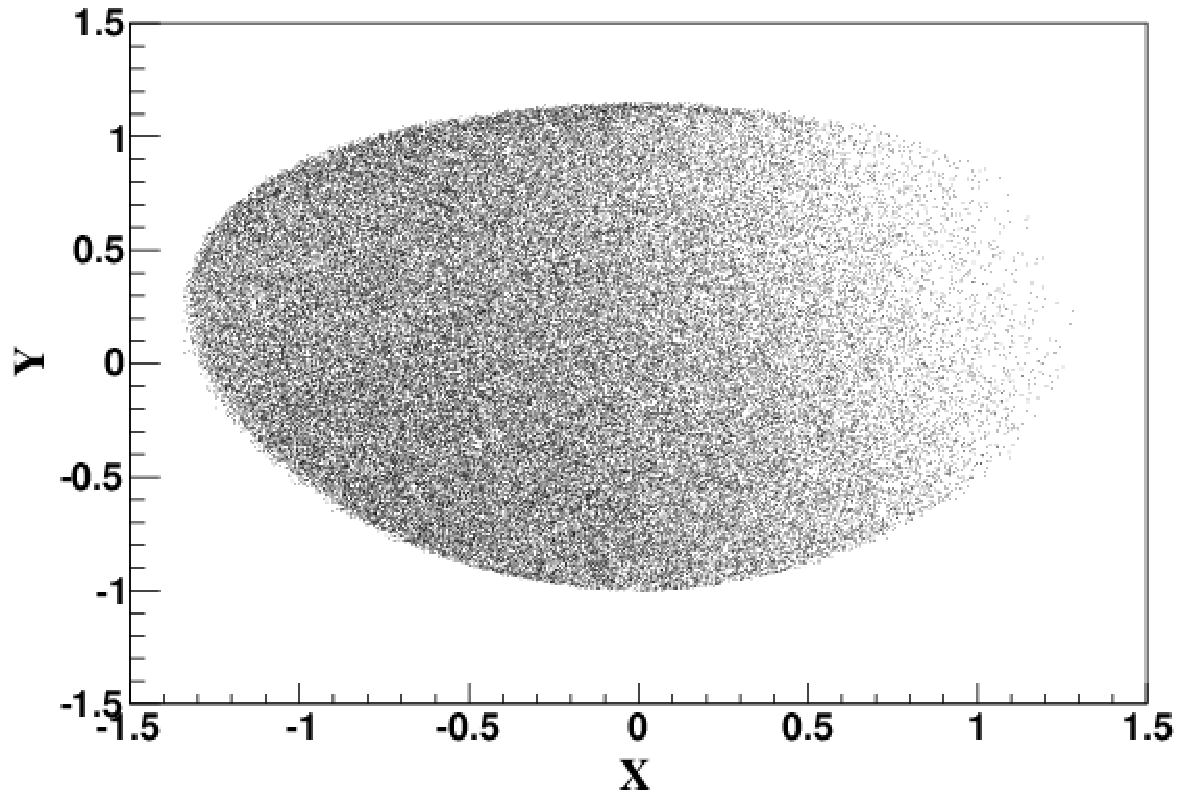
\includegraphics[width=12cm,height=8cm]{dalitzEtaPrime.pdf}}
\caption{Dalitz variable X vs Y for $\eta^{\prime}$ $\rightarrow$ $\eta$ $\pi^{+}$ $\pi^{-}$.}
\label{DP}
\end{figure}

The general parametization function in Equation.~\ref{par} is used to fit a Dalitz plot. The square of the decay amplitude,
 \begin{equation}
M^{2}=A(1+aY+bY^{2}+cX+dX^{2}).
\label{par}
\end{equation}
Where a, b, c, and d are the Dalitz plot parameters of the decay and A is the normalization constant.

The Dalitz plot(DP) provides pure kinematic information of a three body decay and also helps to understand the correct input to theoretical distribution of the effective chiral Lagrangian. A Dalitz plot study for the $\eta^{\prime}$ meson for the $\eta$ $\pi^{+}$ $\pi^{-}$  decay channel will help to study effective chiral perturbation theory at a low Q limit.

The VES Collaboration has reported the Dalitz plot parameters of $\eta^{\prime}$ $\rightarrow$ $\eta$ $\pi^{+}$ $\pi^{-}$ with 14.6 x $10^{3}$ events in charge exchange and 7 x $10^{3}$ events in diffraction like production ~\cite{Dorofeev:2006fb}. The BESIII Collaboration has also reported $\eta^{\prime}$ $\rightarrow$ $\eta$ $\pi^{+}$ $\pi^{-}$ decay parameters with 43826 ± 211 events with better precision~\cite{Ablikim:2010kp}. The two measurements has disagreement among them and also to the theoretical calculation of the parameters ~\cite{Borasoy:2005du}. 

In this note the Dalitz plot parameters of $\eta^{\prime}$ $\rightarrow$ $\eta$ $\pi^{+}$ $\pi^{-}$ is studied with CLAS g12 data set, which has the competitive statistics to study the parameters with low statistical errors. It is yet another independent measurement with different systematic errors to cross-check the parameters.
